\documentclass[11pt, oneside]{article}   	% use "amsart" instead of "article" for AMSLaTeX format
\usepackage[margin=1.0in]{geometry}                		% See geometry.pdf to learn the layout options. There are lots.
\geometry{letterpaper}                   		% ... or a4paper or a5paper or ... 
%\geometry{landscape}                		% Activate for rotated page geometry
\usepackage[parfill]{parskip}    		% Activate to begin paragraphs with an empty line rather than an indent
\usepackage{graphicx}				% Use pdf, png, jpg, or eps§ with pdflatex; use eps in DVI mode
								% TeX will automatically convert eps --> pdf in pdflatex	
									
\usepackage{amssymb}

%SetFonts

%SetFonts

							% Activate to display a given date or no date
\begin{document}

\begin{titlepage}
    \centering
    \vfill
    {\bfseries\Large
        Assignment4: Harris Corner Detection\\
        \vskip2cm
        Suozhi Qi\\
        2/20/17\\
    }    
    \vfill
    \includegraphics[width=50mm]{../../../../../Desktop/selfie.jpg}
    \vfill
    \vfill
\end{titlepage}

\section{Implementation}
\subsection{"Cornerness" measure}
\paragraph{(a)} Please refer to my matlab file. Image is shown below.
\begin{center}
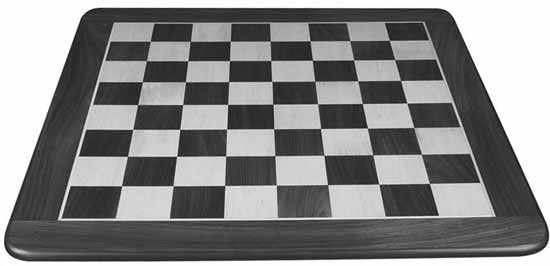
\includegraphics[width=100mm]{../../../../../Desktop/imchessboardgray.png}
\end{center}

\paragraph{(b)} I use the central different filters designed in HW01. X-filter: 1/2 * [-1, 0, 1], y-filter: 1/2 * [-1; 0; 1], and manually filter the gray scale image to get the $I_{x}$ and $I_{y}$. Please refer to my matlab code. Images are shown below.
\begin{center}
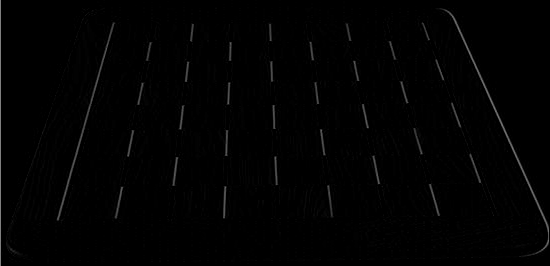
\includegraphics[width=100mm]{../../../../../Desktop/chessboardIx.png}
\newline{}chessboard$I_{x}$\newline\newline
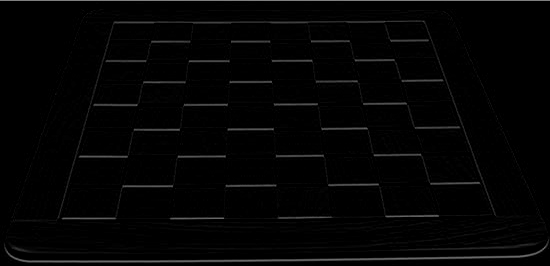
\includegraphics[width=100mm]{../../../../../Desktop/chessboardIy.png}
\newline{}chessboard$I_{y}$\newline\newline
\end{center}

\paragraph{(c)} Please refer to my matlab code. 

\paragraph{(d)} After testing, I choose $\sigma$ to be 2, and the size of the Gaussian filter is therefore 8. Please refer to my matlab code.

\paragraph{(e)} Please refer to my matlab code. Images are shown below.
\begin{center}
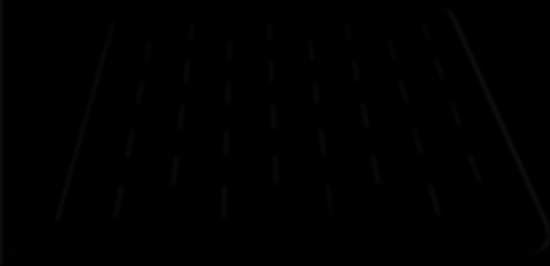
\includegraphics[width=100mm]{../../../../../Desktop/chessboardIx2.png}
\newline{}chessboard$I_{x}^2$\newline\newline

\includegraphics[width=100mm]{../../../../../Desktop/chessboardIy2.png}
\newline{}chessboard$I_{y}^2$\newline\newline

\includegraphics[width=100mm]{../../../../../Desktop/chessboardIxIy.png}
\newline{}chessboard$I_{x}I_{y}$\newline\newline
\end{center}

\paragraph{(f)} Please refer to my matlab code. Image is shown below.
\begin{center}
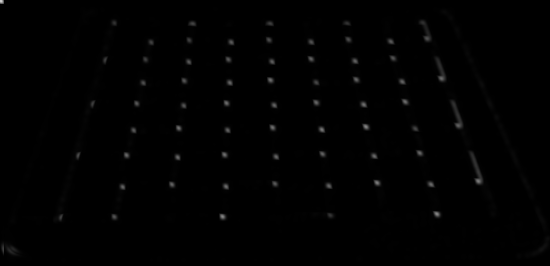
\includegraphics[width=100mm]{../../../../../Desktop/cornerness.png}
\newline{}Cornerness Measure M\newline\newline
\end{center}

\subsection{Corner extraction}
\paragraph{(a)} I use the function ordfilt2 to get the local maximum, and then perform matrix calculation to filter out those that are not maximum, generating single dots. Please refer to my matlab code. Image is shown below.
\begin{center}
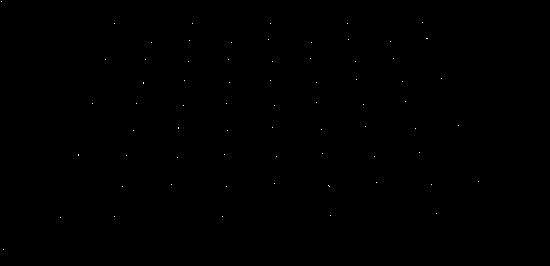
\includegraphics[width=100mm]{../../../../../Desktop/cornerdetect.png}
\newline{}Corner detect\newline\newline
\end{center}

\paragraph{(b)} I use the find function to find the coordinates of the corner points. Please refer to my matlab code for implementation details. \newline
\newline
$I_{x}$: 2
250
218
155
156
104
60
24
217
187
156
131
104
83
84
60
43
185
158
128
129
106
81
62
41
24
217
155
104
187
131
60
83
43
40
24
81
62
128
106
184
157
59
43
83
103
130
154
186
187
216
24
40
62
80
105
127
157
183
42
59
82
102
129
153
23
39
39
185
214
79
126
182 \newline
\newline
$I_{y}$: 2
4
61
79
79
93
106
115
115
123
127
134
137
144
144
146
152
172
178
179
179
184
185
189
190
193
223
225
227
227
228
229
230
232
269
271
271
273
273
275
275
277
311
312
317
317
322
323
329
330
331
348
349
356
357
364
366
375
377
391
394
403
406
416
420
423
427
428
432
437
442
459
479

\paragraph{(c)} Below is the superimposed image. Corners are marked with blue dots. \newline\newline
\begin{center}
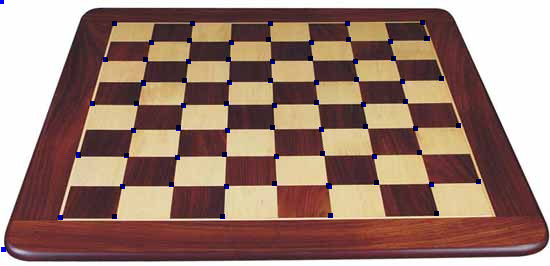
\includegraphics[width = 100mm]{../../../../../Desktop/superimpose.png}
\end{center}
\section{Rotation and Scaling}
\paragraph{Rotate} Below is the rotated image.\newline\newline
\begin{center}
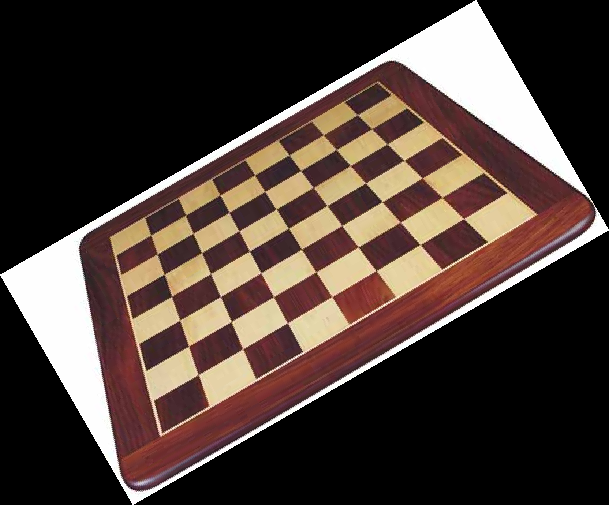
\includegraphics[width = 100mm]{../../../../../Desktop/rotateimg.png}
\end{center}
Below is the superimposed image using the function created above. The original image has been rotated for 30 degrees. Please refer to my matlab code for implementation details.
\newline\newline
\begin{center}
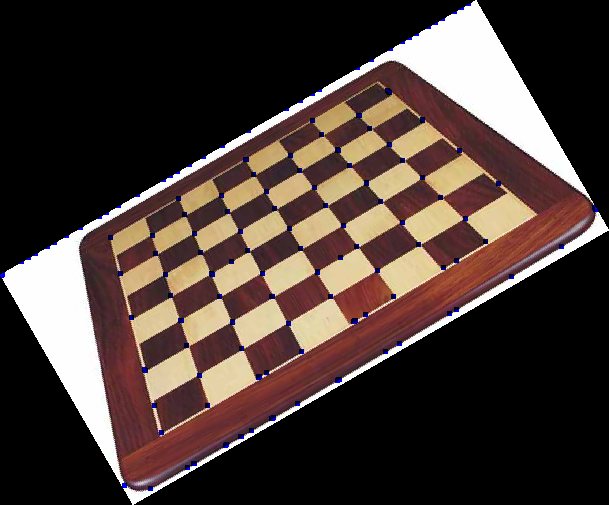
\includegraphics[width = 100mm]{../../../../../Desktop/rotateimpose.png}
\end{center}
\paragraph{Resize} Below is the resized image using the function created above. The original image has been scaled to 4 times bigger. The image on the PDF has been resized for displaying purpose.\newline\newline
\begin{center}
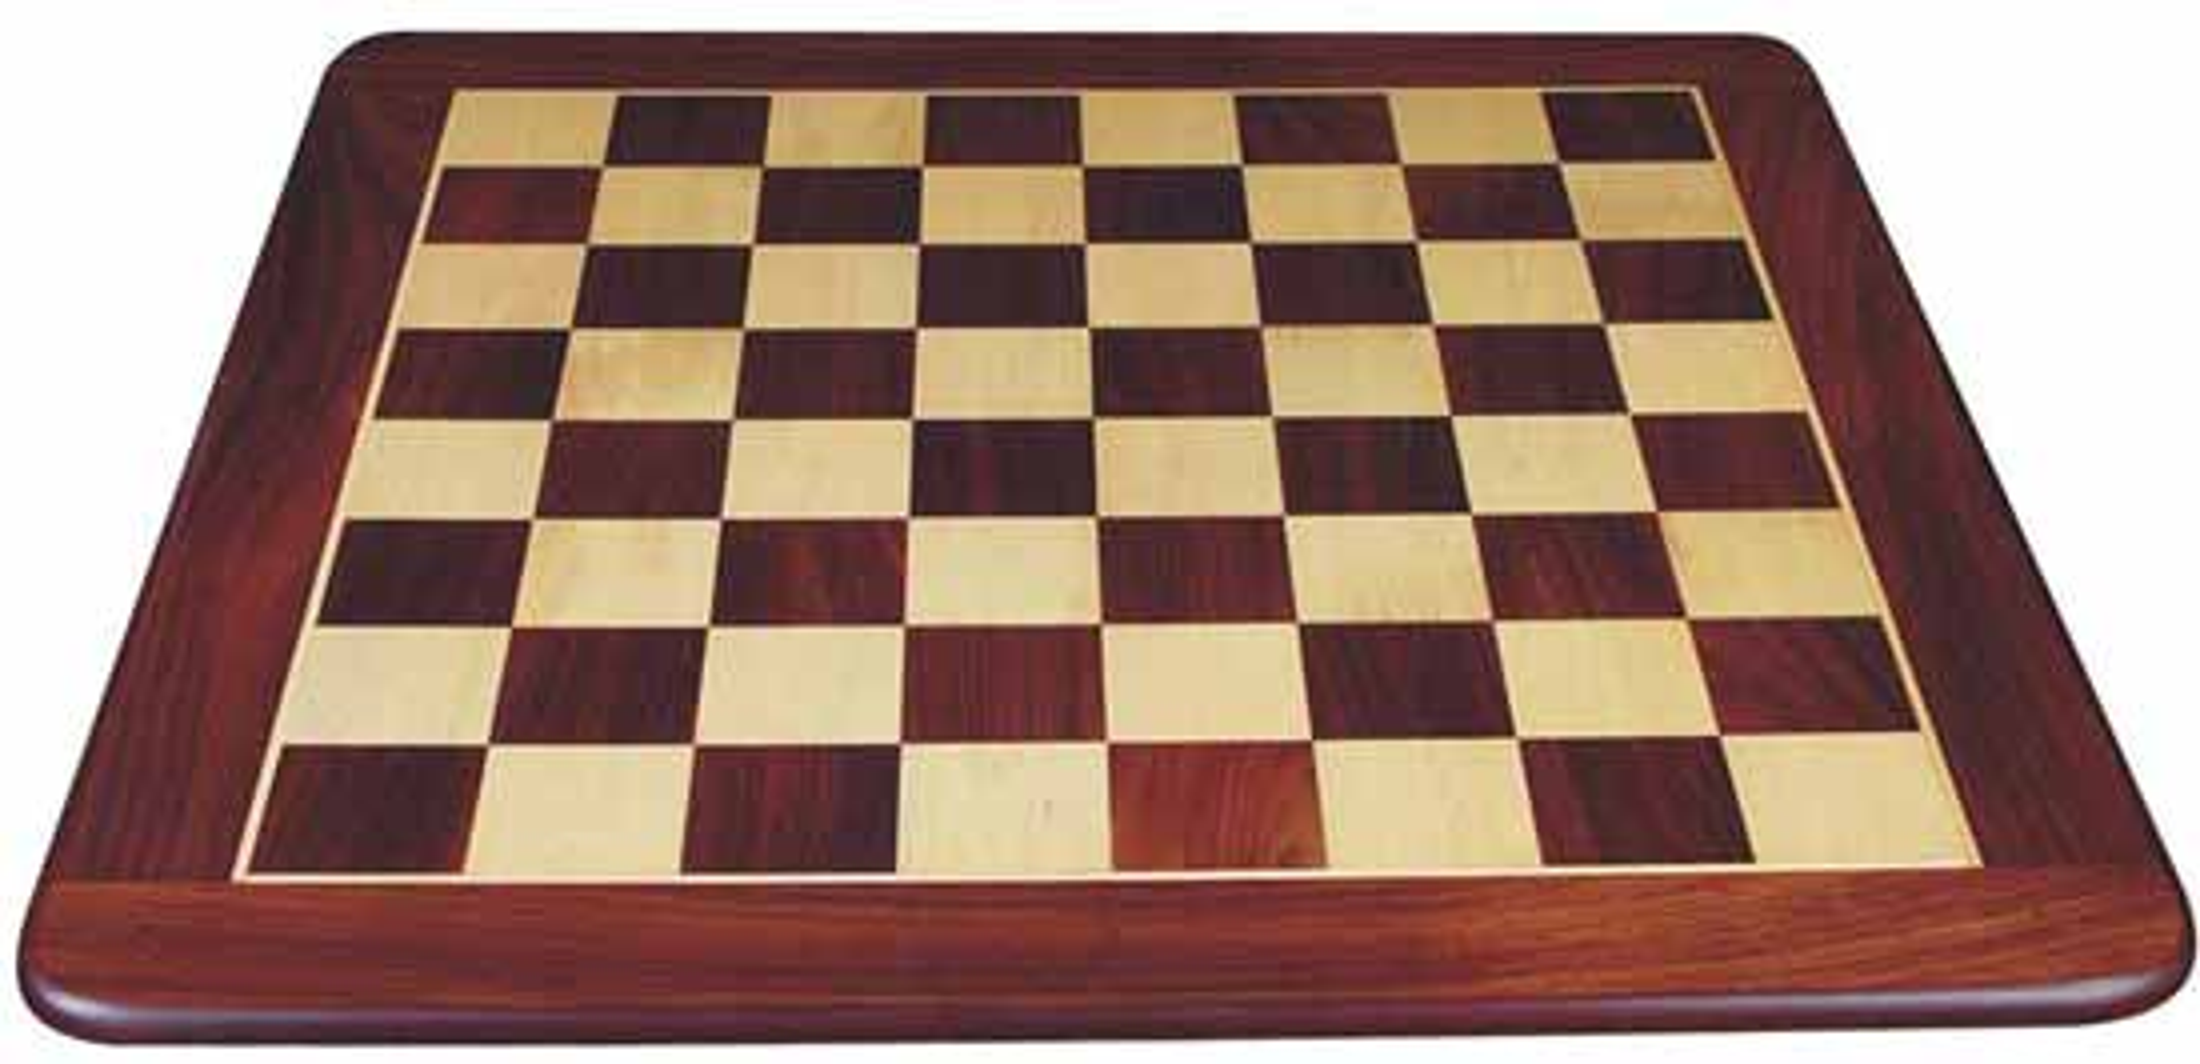
\includegraphics[width = 100mm]{../../../../../Desktop/resizeimg.png}
\end{center}
Below is the superimposed image using the function created above. The original image has been scaled to 4 times bigger. The image on the PDF has been resized for displaying purpose. Please refer to my matlab code for implementation details.
\newline\newline
\begin{center}
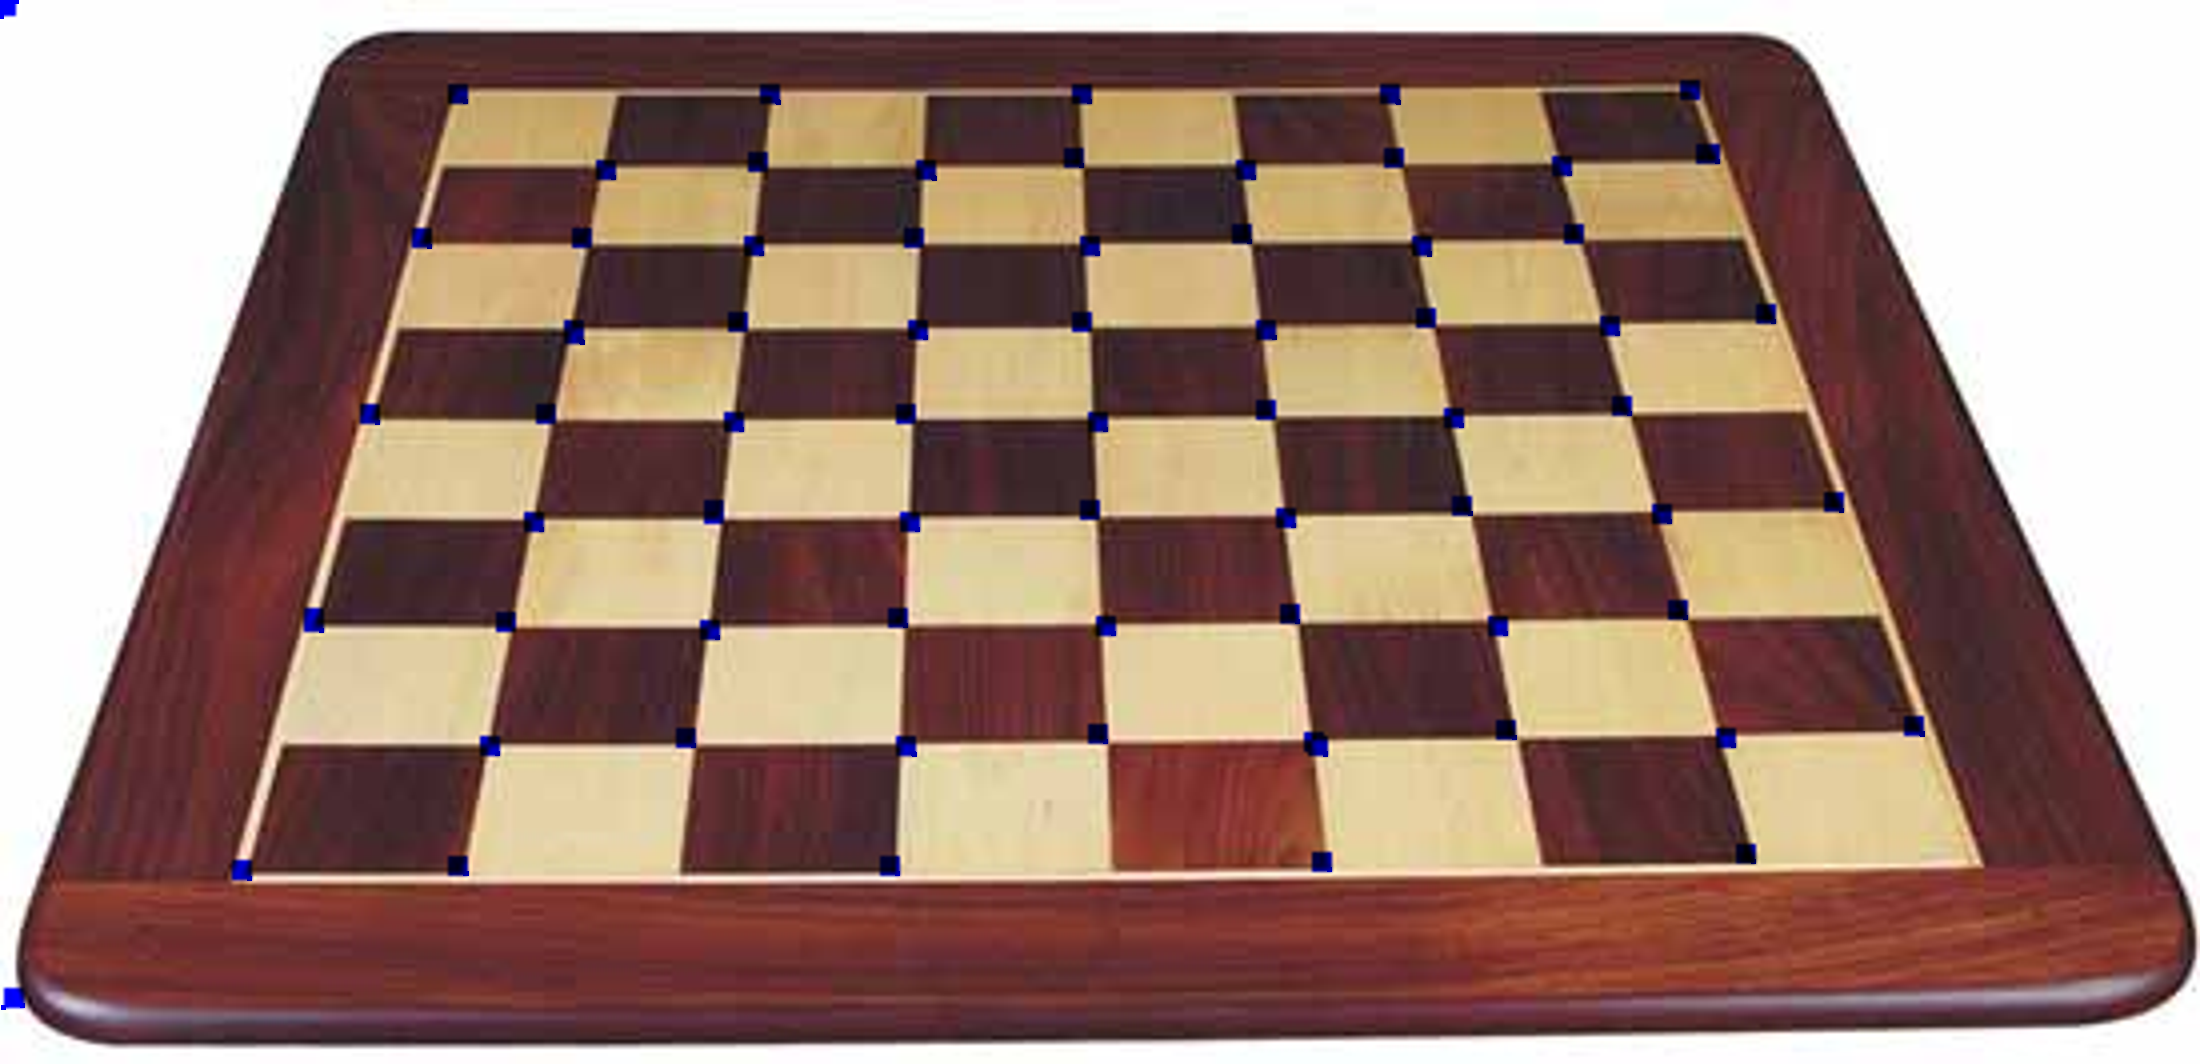
\includegraphics[width = 100mm]{../../../../../Desktop/resizeimpose.png}
\end{center}
\paragraph{Discussion}It looks to me that both the rotated image and the resized image have been corrected processed to detect corners. In the rotated image, we can see more "false" corners being detected at the boarders. This is probably because after rotation, I have created a lot of black parts. Thus at the boarder between the black part and the image, the differences in gradient is big, creating a lot of false positives.\newline 
In the resized image, the result of detection is almost the same as the original one without changing any parameters. This is actually a surprising result for me since I know that after we resize the image to a bigger size, the corners will become less "sharp", thus reducing the ability of Harris corner detector to detect corners. In this case, it's possible that a 4 times enlargement is not enough to make the corners undetectable in my case of parameters.

\section{Grad Credits: SURF}
\begin{center}
SURF: Speeded up Robust Features
\end{center}
\paragraph{}It has been a long-term question in the field of computer vision to find correspondences between images of the same scene. In order to find discrete image correspondences, three major steps should be followed. First of all, interest points should be selected at various locations in the image. These points are selected by detectors and the most important feature of a detector is its repeatability, which means a detector should reproducibly find the same interest point under different viewing environment. Second, the surrounding feature vectors of an interest point are called descriptors. They are supposed to be distinctive and robust to noise and errors. Finally, a matching step is applied to descriptors within different images based on distance calculation. In this paper, the authors proposed modified algorithms and model that focus on scale invariance and lead to more efficient detectors and descriptors but still keep them distinctive and repeatable.
\paragraph{}Many state-of-the-art detectors and descriptors are described in literatures. So far, the most popular detector is the Harris corner detector, which is based on the eigenvalues of the second-moment matrix. However, Harris is not scale-invariant, which makes it less stable. Another researcher proposed the Hessian detector based on automatic scale selection. Hessian is then further modified to become more repeatable and robust. In terms of descriptors, feature descriptors focusing on the distribution of smaller-scale features (SIFT) perform better than other descriptors. SIFT becomes even faster and more distinctive after refinement. Nevertheless, SIFT and its variants possess high dimensionality in the matching step.
\paragraph{}In this paper, the authors proposed a new detector-descriptor set made up of a ``Fast-Hessian" detector and a SURF descriptor with less dimension and less computational time. The Fast-Hessian detector is based on Hessian detector with the discretized and cropped Gaussian filters replaced by box filters. This is because aliasing always occur as long as the resulting images are sub-sampled. Furthermore, box filters are combined with integral images, which change the scale space analysis method from reducing image size repeatedly to up-scaling the filter size. When compared with the SIFT descriptor, the SURF descriptors proposed in this paper further break down the complexity in two steps. The first step is to fix the rotation. Researchers calculate the Haar-wavelet responses of a certain radius 6s around an interest point. s is the scale where the interest point is detected. In such way, only 6 operations are needed to calculate the wavelet response. The response is further computed and weighted to find the dominant orientation. The second step is to build a region aligned to the dominant orientation and extract the SURF descriptor from it. In order to fulfill this step, the constructed region is broken down into 4X4 sub-regions. Within each sub-region, a few simple features are computed with horizontal and vertical Haar wavelet responses calculated. These distances are weighted by Gaussian to increase robustness. A multi-dimensional descriptor vector is then calculated. Various parameters are tested to get the most distinctive descriptors with less dimensionality. The 4X4 sub-regions with 64 dimensions perform the best. In the matching step, indexing with the sign of Laplacian is added without extra computational cost. It distinguishes bright blobs in dark backgrounds from the opposite situation. The actual matching only considers features if they have the same type of contrast, which reduces matching time but increases performance.
\paragraph{}SURF$'$s performance is tested with both standard evaluation and real world recognition application. For the standard evaluation, zoon and rotation as well as lighting changes are tested. The proposed Fast-Hessian detector performs 5 times faster than other modified Hessian detectors with same level of repeatability. The SURF descriptors outperform other descriptors in a significant way. For the object recognition test, SURF descriptor behaves at least 5\% more accurate than other major descriptors. Overall, SURF detectors and descriptors are faster and more accurate than other schemes.  

\end{document}  